\chapter{Rozdmuchania i rozwiązywanie osobliwości}
\label{ch:ga5-rozdmuchania}

\section{Dlaczego wygładzanie osobliwości wymaga zmiany przestrzeni?}
\label{sec:ga5-motywacja}

Rozważmy krzywą $C=\V(y^2-x^3)\subseteq\A^2_\C$. W początku układ
$y^2=x^3$ nie wyznacza gładkiej krzywej: obie pochodne cząstkowe
znikają. Nie jest to jednak argument, że nie można jej opisać
\emph{gładką} krzywą. Parametryzacja $t\mapsto(t^2,t^3)$ pokazuje, że
trudność polega na sposobie umieszczenia krzywej w płaszczyźnie.

Samo usunięcie punktu osobliwego nie jest rozwiązaniem: gubimy punkt,
a zależy nam na odwzorowaniu do wyjściowej krzywej, które nie zmienia
jej poza osobliwościami. Chcemy zastąpić punkt dodatkowymi danymi,
na przykład kierunkiem, z którego do niego dochodzimy. Prowadzi to
do \emph{rozdmuchania} (ang. \emph{blow-up}).

W rozdziale odróżniamy trzy cele:
\begin{enumerate}[label=\arabic*)]
\item \emph{rozdmuchanie otoczenia} punktu w gładkiej powierzchni;
      nowa powierzchnia może nadal być gładka, mimo że włókno nad
      punktem zawiera całą prostą rzutową;
\item \emph{rozwiązanie osobliwości krzywej}: uzyskanie gładkiej
      krzywej z odwzorowaniem właściwym i biwymiernym na $C$;
\item \emph{rozwiązanie zanurzone}: dodatkowo wymaga, aby wygładzona
      krzywa i dzielniki wyjątkowe przecinały się z normalnymi
      skrzyżowaniami.
\end{enumerate}
Trzecie zadanie jest silniejsze od drugiego. Pokażemy to rachunkiem
na ostrzu $y^2=x^3$.

W całym rozdziale $k$ oznacza ciało algebraicznie domknięte
charakterystyki $0$, chyba że przy danym twierdzeniu zaznaczono
słabsze założenia. Posługujemy się wcześniejszymi wiadomościami
o pierścieniach, lokalizacji i schematach afinicznych; potrzebne
uzupełnienia podajemy poniżej. Nie zakładamy znajomości ogólnej
teorii schematów projektowych.

\section{Schematy i morfizmy: minimalny, ale dokładny fundament}
\label{sec:ga5-schematy}

\subsection{Morfizmy i włókna nie są tylko odwzorowaniami punktów}

\begin{definicja}[Morfizm schematów]
\label{def:ga5-morfizm}
Niech $(X,\mathcal O_X)$ i $(Y,\mathcal O_Y)$ będą schematami.
Morfizmem $f:X\to Y$ nazywamy parę złożoną z ciągłego odwzorowania
$f:|X|\to|Y|$ oraz homomorfizmu snopów pierścieni
$f^\sharp:\mathcal O_Y\to f_*\mathcal O_X$ (równoważnie,
$f^{-1}\mathcal O_Y\to\mathcal O_X$), taką że dla każdego $x\in X$
indukowany homomorfizm lokalnych pierścieni
$\mathcal O_{Y,f(x)}\to\mathcal O_{X,x}$ jest \emph{lokalny}, tzn.
przeciwobraz ideału maksymalnego pierścienia $\mathcal O_{X,x}$
jest dokładnie ideałem maksymalnym $\mathcal O_{Y,f(x)}$.
\end{definicja}

Sformułowanie „homomorfizm lokalny” oznacza dokładnie
$\varphi^{-1}(\mathfrak m_B)=\mathfrak m_A$ dla homomorfizmu
$\varphi:A\to B$ pierścieni lokalnych $(A,\mathfrak m_A)$ i
$(B,\mathfrak m_B)$. Dzięki temu odwzorowanie respektuje funkcje
regularne i ich wartości, a nie tylko zbiór punktów.

\begin{stwierdzenie}[Morfizmy schematów afinicznych]
\label{st:ga5-affine-morphism}
Dla dowolnych pierścieni przemiennych $A,B$ z jedynką istnieje
naturalna bijekcja
\[
 \operatorname{Hom}_{\mathrm{Sch}}(\Spec B,\Spec A)
 \cong\operatorname{Hom}_{\mathrm{Ring}}(A,B).
\]
Homomorfizm $\varphi:A\to B$ odpowiada odwzorowaniu
$\mathfrak q\mapsto\varphi^{-1}(\mathfrak q)$ na ideałach pierwszych.
\end{stwierdzenie}
\begin{proof}
Przeciwobraz ideału pierwszego jest pierwszy: jeśli
$\varphi(a)\varphi(b)\in\mathfrak q$, to przynajmniej jeden
z obrazów należy do $\mathfrak q$. Ponadto
$\varphi^{-1}(D(a))=D(\varphi(a))$, więc odwzorowanie spektrów
jest ciągłe. Na podstawowych otwartych zbiorach $D(a)$
homomorfizm $A\to B$ indukuje
$A_a\to B_{\varphi(a)}$ przez $u/a^m\mapsto\varphi(u)/\varphi(a)^m$.
Te homomorfizmy są zgodne z dalszymi lokalizacjami i sklejają się
do homomorfizmu snopów. Na źdźbłach dostajemy
$A_{\mathfrak p}\to B_{\mathfrak q}$ dla
$\mathfrak p=\varphi^{-1}(\mathfrak q)$; jest to homomorfizm lokalny.

W drugą stronę morfizm schematów określa homomorfizm sekcji
globalnych $\Gamma(\Spec A,\mathcal O)=A\to
\Gamma(\Spec B,\mathcal O)=B$. Dla $\mathfrak q\in\Spec B$
lokalność homomorfizmu na źdźbłach wymusza obraz
$\varphi^{-1}(\mathfrak q)$. Zgodność z ograniczeniami do
$D(a)$ wymusza również opisany homomorfizm snopów.
Zatem obie konstrukcje są wzajemnie odwrotne.
\end{proof}

\begin{przyklad}[Dlaczego kierunek strzałki się odwraca?]
Homomorfizm $k[t]\to k[x]$, $t\mapsto x^2$, daje morfizm
$\A^1_k\to\A^1_k$ wysyłający $a\mapsto a^2$ na punktach
zamkniętych. Funkcje na przestrzeni docelowej cofamy na przestrzeń
źródłową: $t$ staje się funkcją $x^2$.
Ta kontrawariantność nie jest kwestią zapisu, lecz zasadą
geometryczną „funkcję można złożyć z odwzorowaniem”.
\end{przyklad}

\begin{definicja}[Iloczyn włóknisty i włókno]
\label{def:ga5-fibreproduct}
Dla morfizmów $f:X\to S$ i $g:Y\to S$ ich \emph{iloczynem
włóknistym} jest schemat $X\times_S Y$ wraz z rzutowaniami do $X$
i $Y$, komutującymi z odwzorowaniami do $S$, o następującej
własności uniwersalnej: każdy schemat $T$ z morfizmami $T\to X$
i $T\to Y$ zgodnymi po przejściu do $S$ ma dokładnie jeden
morfizm $T\to X\times_S Y$ zgodny z rzutowaniami.

Jeżeli $s\in S$ i $\kappa(s)$ oznacza ciało reszt
$\mathcal O_{S,s}/\mathfrak m_s$, to \emph{włóknem} $f$ nad $s$
jest schemat $X_s=X\times_S\Spec\kappa(s)$.
\end{definicja}

\begin{stwierdzenie}[Iloczyn włóknisty w przypadku afinicznym]
\label{st:ga5-tensor-fibre}
Dla homomorfizmów $R\to A$, $R\to B$ zachodzi
\[
 \Spec A\times_{\Spec R}\Spec B\cong\Spec(A\otimes_R B).
\]
\end{stwierdzenie}
\begin{proof}
Dla dowolnego pierścienia $C$ homomorfizm
$A\otimes_R B\to C$ odpowiada parze homomorfizmów
$A\to C$ i $B\to C$, których ograniczenia do $R$ są równe:
para wyznacza odwzorowanie $a\otimes b\mapsto\alpha(a)\beta(b)$,
a jego istnienie i jednoznaczność wynika z własności uniwersalnej
iloczynu tensorowego. Za pomocą stwierdzenia~\ref{st:ga5-affine-morphism}
jest to dokładnie własność uniwersalna iloczynu włóknistego
schematów afinicznych. Dla dowolnego schematu $T$ parę
morfizmów $T\to\Spec A$ i $T\to\Spec B$ zgodnych nad
$\Spec R$ ograniczamy do jego afinicznego pokrycia.
Na każdym otwartym afinicznym otrzymujemy jedyny morfizm
w $\Spec(A\otimes_R B)$; jednoznaczność zapewnia ich
zgodność na przecięciach, toteż sklejają się na całym $T$.
Dowodzi to wymaganej własności uniwersalnej bez
ograniczania schematu testowego do przypadku afinicznego.
\end{proof}

\begin{przyklad}[Włókno może być punktem „podwójnym”]
\label{prz:ga5-double-fibre}
W tym przykładzie $k$ jest dowolnym ciałem o charakterystyce różnej od $2$ (nie zakładamy jego algebraicznej domkniętości).
Niech $f:\A^1_k\to\A^1_k$ będzie dany przez $t=x^2$.
Nad punktem $t=0$ otrzymujemy
$\Spec(k[x]\otimes_{k[t]}k[t]/(t))\cong\Spec k[x]/(x^2)$.
To włókno ma jeden punkt topologiczny, ale zawiera niezerowy
nilpotent $\overline x$. Nad $t=a\ne0$ (przy $\operatorname{char}k\ne2$)
włókno jest zredukowanym schematem $\Spec k[x]/(x^2-a)$.
Ma dwa różne punkty $k$-wymierne, jeśli $a$ jest kwadratem
w $k$; jeśli $a$ nie jest kwadratem, wielomian $x^2-a$
jest nierozkładalny i włókno ma jeden punkt o ciele reszt
$k(\sqrt a)$. Po przejściu do domknięcia algebraicznego
włókno ma zawsze dwa różne punkty geometryczne.
Dlatego obraz geometryczny włókna nie zawiera całej informacji
o morfizmie.
\end{przyklad}

\subsection{Zanurzenia zamknięte, ideały i obrazy odwrotne}

\begin{definicja}[Zanurzenie zamknięte i centrum]
Morfizm $i:Z\to X$ jest \emph{zanurzeniem zamkniętym}, gdy
lokalnie na $X=\Spec A$ pochodzi od surjekcji $A\to A/I$.
Wtedy $Z$ jest \emph{podschematem zamkniętym} wyznaczonym
przez snop ideałów $\mathcal I\subseteq\mathcal O_X$.
Przeciwobrazem schematowym $f^{-1}(Z)$ względem $f:Y\to X$
nazywamy $Y\times_X Z$; jego snop ideałów jest
obrazem $f^*\mathcal I\to\mathcal O_Y$, oznaczanym
$\mathcal I\mathcal O_Y$.
\end{definicja}

\begin{uwaga}[Przeciwobraz zbiorowy i schematowy]
Przeciwobraz zbioru $|Z|$ ma te same punkty co
$|Y\times_X Z|$, lecz nie pamięta krotności. Na przykład
przeciwobraz schematowy zera przez $x\mapsto x^2$
jest właśnie $\Spec k[x]/(x^2)$, nie $\Spec k$.
Ta różnica powróci przy \emph{transformacie całkowitej} krzywej.
\end{uwaga}

\subsection{Gładkość, właściwość i biwymierność}

\begin{definicja}[Gładkość morfizmu]
\label{def:ga5-smooth}
Morfizm schematów $f:X\to S$ jest \emph{gładki w punkcie}
$x\in X$ o wymiarze względnym $d$, jeżeli w pewnych otoczeniach
afinicznych $x$ i $f(x)$ można przedstawić go jako morfizm
$\Spec B\to\Spec R$, gdzie
$B=(R[z_1,\ldots,z_n]/(F_1,\ldots,F_r))_h$,
$n-r=d$ i pewien minor rozmiaru $r$ macierzy
$(\partial F_i/\partial z_j)$ jest odwracalny w $B$.
Morfizm jest \emph{gładki}, jeśli jest gładki w każdym punkcie.
\end{definicja}

Jest to kryterium oparte na \emph{lokalnych prezentacjach
standardowo gładkich}; równoważność z innymi definicjami gładkości
morfizmów wymaga twierdzenia o lokalnym modelu gładkim.
Wynik ten przyjmujemy w ogólnym przypadku. W przykładach poniżej
wystarczą wprost podane prezentacje i rachunek Jacobiego.

\begin{przyklad}[Rodzina gładka poza jednym parametrem]
Dla $X=\V(xy-t)\subseteq\A^2_{x,y}\times\A^1_t$
morfizm $X\to\A^1_t$ ma nad $t=a\ne0$ gładką hiperbolę
$xy=a$, a nad $t=0$ sumę osi $xy=0$. Cała przestrzeń $X$
jest izomorficzna z $\A^2_{x,y}$, lecz morfizm do osi parametru
nie jest gładki w punkcie $(x,y,t)=(0,0,0)$: różniczki
względem zmiennych włókna to $(y,x)$, które tam znikają.
Gładkość całej przestrzeni nie oznacza gładkości każdego morfizmu.
\end{przyklad}

\begin{definicja}[Morfizm właściwy i rzutowy]
\label{def:ga5-proper}
Morfizm schematów $f:X\to S$ jest \emph{właściwy}, gdy jest
skończonego typu, rozdzielony i uniwersalnie domknięty:
dla każdego $S'\to S$ rzutowanie
$X\times_S S'\to S'$ wysyła zbiory domknięte na domknięte.
Morfizm jest \emph{rzutowy}, gdy nad $S$ jest izomorficzny
z zanurzeniem zamkniętym $X\hookrightarrow\PP^n_S$
(złożonym z projekcją $\PP^n_S\to S$) dla pewnego $n$.
\end{definicja}

\begin{uwaga}[Skąd bierze się właściwość?]
Każdy morfizm rzutowy jest właściwy; w ogólności dowód wymaga
kryterium wartościowaniowego i faktu, że $\PP^n_S\to S$ jest
właściwy. Dla czytelnika ważny jest konkretny sens:
morfizm $\A^1_k\to\Spec k$ nie jest właściwy, zaś
$\PP^1_k\to\Spec k$ jest właściwy, choć $\PP^1$ nie jest
afiniczna. Przykładowy dowód wartościowaniowy dla
$\PP^n$ podajemy w stwierdzeniu~\ref{st:ga5-valuative-projective}.
\end{uwaga}

\begin{stwierdzenie}[Rozszerzanie punktów rzutowych nad DVR]
\label{st:ga5-valuative-projective}
Niech $R$ będzie dyskretnym pierścieniem wartościowania,
$K=\Frac(R)$ i $n\ge0$. Każdy punkt $p\in\PP^n(K)$
ma dokładnie jedno przedłużenie do morfizmu
$\Spec R\to\PP^n_R$ zgodnego z $p$ nad $\Spec K$.
\end{stwierdzenie}
\begin{proof}
Weźmy jednorodne współrzędne $p=[a_0:\cdots:a_n]$
z $a_i\in K$, nie wszystkie zerowe. Niech $\pi$ oznacza
parametr jednostajny $R$. Po pomnożeniu wszystkich
$a_i$ przez odpowiednią potęgę $\pi$ możemy założyć,
że wszystkie $a_i\in R$ i co najmniej jeden z nich jest
jednostką. Dają zatem morfizm $\Spec R\to\PP^n_R$:
na otoczeniu $D_+(X_i)$ wybranego odwracalnego $a_i$
współrzędne afiniczne mają wartości $a_j/a_i\in R$.

Jeśli $[b_0:\cdots:b_n]$ określa inne przedłużenie,
możemy analogicznie wybrać współrzędne całkowite z
co najmniej jedną jednostką. Na punkcie ogólnym mamy
$b_i=\lambda a_i$ dla wspólnego $\lambda\in K^\times$.
Minimalne wartościowania współrzędnych obu reprezentacji
są równe zeru, więc $v(\lambda)=0$: $\lambda$ jest
jednostką $R$. Wobec tego obie reprezentacje wyznaczają
ten sam morfizm. Jest to część kryterium wartościowaniowego,
która wyjaśnia geometrycznie, dlaczego granice kierunków
pozostają w przestrzeni rzutowej.
\end{proof}

\begin{definicja}[Morfizm biwymierny i rozwiązanie osobliwości]
\label{def:ga5-resolution}
Niech $X,Y$ będą całkowitymi (nierozkładalnymi i zredukowanymi)
schematami skończonego typu nad $k$. Morfizm $f:Y\to X$
nazywamy \emph{biwymiernym}, jeśli indukuje izomorfizm ciał
funkcji $k(X)\cong k(Y)$; równoważnie istnieją niepuste
otwarte podzbiory, na których $f$ jest izomorfizmem.
\emph{Rozwiązaniem osobliwości} całkowitego schematu $X$
nazywamy właściwy morfizm biwymierny $\pi:\widetilde X\to X$,
gdzie $\widetilde X$ jest gładka nad $k$, a $\pi$ jest
izomorfizmem nad gładkim miejscem $X_{\mathrm{reg}}$.
\end{definicja}

Warunek „właściwy” zapobiega uznaniu samego otwartego
podzbioru gładkiego za rozwiązanie. Wymaganie izomorfizmu
nad $X_{\mathrm{reg}}$ zapobiega niepotrzebnemu zmienianiu
gładkich punktów. W dalszym ciągu będziemy rozpatrywać
także podschematy zredukowane o wielu składowych;
wtedy rozwiązuje się oddzielnie składowe lub używa
odpowiedniej wersji dla schematów zredukowanych.

\section{Konstrukcja \texorpdfstring{$\operatorname{Proj}$}{Proj}: przestrzeń z algebry stopniowanej}
\label{sec:ga5-proj}

\begin{definicja}[Spektrum jednorodne]
Niech $S=\bigoplus_{n\ge0}S_n$ będzie pierścieniem
stopniowanym, $S_mS_n\subseteq S_{m+n}$, i niech
$S_+=\bigoplus_{n>0}S_n$ będzie ideałem nieistotnym
(ang. \emph{irrelevant ideal}). Definiujemy
\[
 \operatorname{Proj}S=
 \{\mathfrak p\subset S:\mathfrak p\text{ jest jednorodnym ideałem
 pierwszym},\ S_+\not\subseteq\mathfrak p\}.
\]
Dla jednorodnego $f\in S_d$, $d>0$, oznaczamy
$D_+(f)=\{\mathfrak p\in\operatorname{Proj}S:f\notin\mathfrak p\}$.
\end{definicja}

Ideał jednorodny oznacza ideał generowany przez elementy
jednorodne. Pominięcie ideałów zawierających $S_+$ jest
istotne: w $k[T_0,T_1]$ ideał $(T_0,T_1)$ odpowiadałby
początkowi stożka, a nie kierunkowi na prostej rzutowej.

\begin{definicja}[Część stopnia zerowego lokalizacji]
Jeżeli $f\in S_d$ jest jednorodny, $d>0$, to
$S_{(f)}=(S_f)_0$ oznacza podpierścień elementów stopnia
$0$ w lokalizacji $S_f$. Każdy jego element można zapisać
jako $a/f^m$, gdzie $a\in S_{md}$ jest jednorodny.
\end{definicja}

\begin{stwierdzenie}[Podstawowe otwarte w $\operatorname{Proj}$]
\label{st:ga5-proj-charts}
Dla każdego jednorodnego $f\in S_+$ przestrzeń $D_+(f)$
ma kanoniczną strukturę schematu afinicznego
$D_+(f)\cong\Spec S_{(f)}$. Jeśli $S$ jest generowany
jako $S_0$-algebra przez skończenie wiele elementów
$f_1,\ldots,f_r$ dodatnich stopni, to zbiory $D_+(f_i)$
pokrywają $\operatorname{Proj}S$.
\end{stwierdzenie}
\begin{proof}
Wzajemne przyporządkowanie ideałów pierwszych uzyskuje się
przez lokalizację jednorodnych ideałów $\mathfrak p$
niezawierających $f$, a następnie wzięcie ich części
stopnia zero. W drugą stronę dla
$\mathfrak q\in\Spec S_{(f)}$ rozważa się jednorodne
$a\in S_e$, których odpowiednia potęga $a^d/f^e$
należy do $\mathfrak q$. Użycie potęg jest potrzebne,
gdy $\deg f>1$. Z definicji wynika, że otrzymany zbiór
jest jednorodnym ideałem pierwszym, niezawierającym $f$;
obie operacje są odwrotne. Lokalizacje funkcji regularnych
na dalszych otwartych podzbiorach są zgodne, co daje
strukturę snopa i identyfikację schematów afinicznych.

Jeśli $\mathfrak p\in\operatorname{Proj}S$ zawierałby
wszystkie $f_i$, to zawierałby również generowany
przez nie ideał $S_+$, wbrew definicji. Zatem
przynajmniej jedno $f_i$ nie należy do $\mathfrak p$
i otrzymujemy pokrycie.
\end{proof}

\begin{przyklad}[Powrót do zwykłej przestrzeni rzutowej]
Dla $S=k[U,V]$ ze zwykłym stopniowaniem
$D_+(U)=\Spec k[V/U]$, a $D_+(V)=\Spec k[U/V]$.
Na przecięciu współrzędne $v=V/U$ i $u=U/V$
spełniają $uv=1$. Sklejenie dwóch prostych afinicznych
według $u=v^{-1}$ daje $\PP^1_k$.
Podobnie $\operatorname{Proj}k[T_0,\ldots,T_n]=\PP^n_k$.
\end{przyklad}

\begin{uwaga}[Co jest tu twierdzeniem, a co konstrukcją?]
Pełne sprawdzenie zgodności snopów na przecięciach jest
standardowym lematem konstrukcji $\operatorname{Proj}$.
Dla rozdmuchań będziemy korzystać tylko z jawnych map
opisanych pierścieniami i sprawdzimy ich przejścia bezpośrednio.
Dlatego dalsze rachunki nie zależą od nieudowodnionych
własności kohomologicznych $\operatorname{Proj}$.
\end{uwaga}

\section{Algebra Reesa i właściwa definicja rozdmuchania}
\label{sec:ga5-rees}

\begin{definicja}[Algebra Reesa]
\label{def:ga5-rees}
Niech $A$ będzie pierścieniem przemiennym z jedynką,
a $I\subseteq A$ ideałem. Jego \emph{algebrą Reesa}
nazywamy pierścień stopniowany
\[
 \mathcal R_A(I)=\bigoplus_{n\ge0}I^nT^n\subseteq A[T],
 \qquad I^0=A,
\]
przy czym składnik $I^nT^n$ ma stopień $n$.
\emph{Rozdmuchaniem} $\Spec A$ wzdłuż centrum
$Z=\Spec(A/I)$ jest schemat
$\operatorname{Bl}_Z(\Spec A)=\operatorname{Proj}\mathcal R_A(I)$
z naturalnym morfizmem $\pi:\operatorname{Bl}_Z(\Spec A)\to\Spec A$.
\end{definicja}

\begin{uwaga}[Dlaczego nie wystarczy $A/I$?]
Iloraz $A/I$ pamięta samo centrum. Ciąg
$I,I^2,I^3,\ldots$ pamięta kolejne rzędy znikania
wzdłuż centrum. Algebra Reesa zbiera je w jednym
obiekcie stopniowanym. Po wzięciu $\operatorname{Proj}$
uzyskujemy kierunki, w jakich znikają elementy $I$.
To właśnie informacja tracona przy zastąpieniu
centrum pojedynczym punktem.
\end{uwaga}

\begin{stwierdzenie}[Mapy współrzędnych rozdmuchania dziedziny]
\label{st:ga5-blowup-charts}
Niech $A$ będzie dziedziną, a
$I=(f_1,\ldots,f_r)\ne(0)$ ideałem skończenie generowanym,
przy czym $f_i\ne0$. Rozdmuchanie $\operatorname{Bl}_I\Spec A$
jest pokryte przez mapy
\[
 U_i=\Spec A[I/f_i],\qquad
 A[I/f_i]=A\bigl[f_1/f_i,\ldots,f_r/f_i\bigr]\subseteq\Frac(A).
\]
Na $U_i$ ideał centrum po cofnięciu staje się główny:
$I\mathcal O_{U_i}=f_i\mathcal O_{U_i}$.
\end{stwierdzenie}
\begin{proof}
Algebra Reesa jest generowana nad $A$ przez jednorodne
elementy $f_1T,\ldots,f_rT$. Zatem z poprzedniego
stwierdzenia wystarczą $D_+(f_iT)$. Element stopnia
zero w $\mathcal R_A(I)_{f_iT}$ ma postać
$(aT^m)/(f_iT)^m=a/f_i^m$ dla $a\in I^m$.
Ponieważ $A$ jest dziedziną, traktujemy te ilorazy
jako elementy $\Frac(A)$. Są generowane przez $A$
oraz $f_j/f_i$, więc pierścień mapy to $A[I/f_i]$.
Dla każdego $j$ równość $f_j=f_i(f_j/f_i)$ pokazuje,
że $I\mathcal O_{U_i}\subseteq f_i\mathcal O_{U_i}$;
odwrotna inkluzja jest oczywista, bo $f_i\in I$.
\end{proof}

\begin{uwaga}[Ograniczenie ważne przy dzielnikach zera]
Jeśli $A$ ma dzielniki zera, zapis $A[I/f_i]$ jako
podpierścienia $A_{f_i}$ może zgubić torsję. Ogólne
mapy definiujemy wtedy wyłącznie przez
$(\mathcal R_A(I)_{f_iT})_0$; nie wolno bez dowodu
zastępować ich ilorazami w ciele ułamków.
W szczególności definicja przez algebrę Reesa działa
także dla schematów niezredukowanych.
\end{uwaga}

\begin{stwierdzenie}[Poza centrum nic się nie zmienia]
\label{st:ga5-off-centre}
Dla dowolnego schematu $X$ i quasi-koherentnego snopa
ideałów $\mathcal I$ skończonego typu, definiującego $Z\subseteq X$
morfizm rozdmuchania indukuje izomorfizm
$\operatorname{Bl}_Z X\setminus\pi^{-1}(Z)\cong X\setminus Z$.
\end{stwierdzenie}
\begin{proof}
Wystarczy sprawdzić to po ograniczeniu do otwartych
afinicznych. Jeżeli $f\in I$ jest odwracalne na $D(f)$,
to $I A_f=A_f$. Jego algebra Reesa jest wówczas
$A_f[T]$ ze zwykłym stopniowaniem, więc
$\operatorname{Proj}A_f[T]\cong\Spec A_f$: jedyna mapa
$D_+(T)$ jest całym $\operatorname{Proj}$, a jego
pierścień stopnia zero jest $A_f$. Zbiory $D(f)$
dla $f\in I$ pokrywają dopełnienie centrum; otrzymane
izomorfizmy są zgodne na przecięciach.
\end{proof}

\begin{stwierdzenie}[Rozdmuchanie jest lokalnie rzutowe i właściwe]
\label{st:ga5-blowup-proper}
Niech $X$ będzie schematem, a $\mathcal I\subseteq\mathcal O_X$
quasi-koherentnym snopem ideałów skończonego typu.
W otoczeniach afinicznych $X$ morfizm rozdmuchania jest
złożeniem zanurzenia zamkniętego w pewną przestrzeń
$\PP^{r-1}_X$ i projekcji na $X$. Zatem jest lokalnie
na bazie rzutowy, a w szczególności właściwy. Istnienie
jednego globalnego zanurzenia w $\PP^N_X$ wymaga
silniejszych założeń i nie wynika wyłącznie z tej lokalnej
konstrukcji.
\end{stwierdzenie}
\begin{proof}
Lokalnie niech $I=(f_1,\ldots,f_r)\subseteq A$.
Przyporządkowanie $T_i\mapsto f_iT$ daje surjektywny
homomorfizm stopniowanych $A$-algebr
$A[T_1,\ldots,T_r]\twoheadrightarrow\mathcal R_A(I)$.
Każdy jednorodny ideał relacji wycina domknięty
podschemat w $\operatorname{Proj}A[T_1,\ldots,T_r]
=\PP^{r-1}_A$; otrzymujemy więc zanurzenie zamknięte
rozdmuchania w przestrzeni rzutowej nad $\Spec A$.
Złożenie zanurzenia zamkniętego z projekcją rzutową
jest właściwe. Ostatnie przejście wykorzystuje standardowe
twierdzenie o właściwości morfizmów rzutowych (jego
mechanizm wartościowaniowy zilustrowaliśmy wcześniej).
\end{proof}

\begin{uwaga}[Drobna, ale istotna subtelność globalna]
Lokalny dowód daje \emph{morfizm lokalnie rzutowy}.
Jeśli ideał $\mathcal I$ jest generowany przez skończoną
rodzinę sekcji globalnych, otrzymujemy globalne zanurzenie
w $\PP^{r-1}_X$. Z właściwości jako własności lokalnej
na bazie wynika jednak, że lokalna rzutowość wystarcza
do właściwości również bez założenia noetherowskości.
Nie należy utożsamiać obu rodzajów rzutowości.
\end{uwaga}

\subsection{Własność uniwersalna i dzielniki Cartiera}

\begin{definicja}[Efektywny dzielnik Cartiera]
\label{def:ga5-cartier}
Podschemat zamknięty $D\subseteq Y$ jest \emph{efektywnym
dzielnikiem Cartiera}, jeżeli jego snop ideałów
$\mathcal I_D$ jest lokalnie generowany przez jeden
\emph{dzielnik regularny}, czyli przez element niebędący
dzielnikiem zera w odpowiednim pierścieniu lokalnym.
Wówczas $\mathcal I_D$ jest snopem odwracalnym.
\end{definicja}

\begin{przyklad}[Dzielnik Cartiera to nie dowolne równanie]
W $\A^2$ prosta $x=0$ jest efektywnym dzielnikiem Cartiera,
bo $x$ nie jest dzielnikiem zera w $k[x,y]$.
Natomiast w $\Spec k[x,y]/(xy)$ element $x$ jest dzielnikiem
zera; podschemat zadany przez $(x)$ nie jest tam efektywnym
dzielnikiem Cartiera. Znaczenie ma pierścień otoczenia,
a nie sam widoczny zbiór punktów.
\end{przyklad}

\begin{twierdzenie}[Własność uniwersalna rozdmuchania]
\label{tw:ga5-universal}
Niech $X$ będzie schematem, $\mathcal I\subseteq\mathcal O_X$
quasi-koherentnym snopem ideałów skończonego typu i
$\pi:\widetilde X=\operatorname{Bl}_{\mathcal I}X\to X$
rozdmuchaniem. Wtedy $\mathcal I\mathcal O_{\widetilde X}$
jest ideałem efektywnego dzielnika Cartiera. Ponadto
każdy morfizm $f:Y\to X$, dla którego
$\mathcal I\mathcal O_Y$ definiuje efektywny dzielnik
Cartiera, faktoryzuje się \emph{jednoznacznie} przez $\pi$:
$ f=\pi\circ\widetilde f$ dla dokładnie jednego
$\widetilde f:Y\to\widetilde X$.
\end{twierdzenie}
\begin{proof}
Własność jest lokalna na $X$ i $Y$. Na otoczeniu
afinicznym $X=\Spec A$ niech $I=(f_1,\ldots,f_r)$.
Na mapie $D_+(f_iT)$ ideał $I\mathcal O_{\widetilde X}$
jest generowany przez obraz $f_i$. Musimy uzasadnić,
że jest on niedzielnikiem zera również wtedy, gdy $A$
nie jest dziedziną. Oznaczmy przez $B_i$ część stopnia
zero $\mathcal R_A(I)_{f_iT}$. Jeśli $f_i b=0$ w $B_i$,
wybierzmy zapis $b=aT^m/(f_iT)^m$ z $a\in I^m$.
Zerowość $f_i b$ w lokalizacji znaczy, że istnieje
$N\ge0$ takie, że $(f_iT)^N(f_i aT^m)=0$
w $\mathcal R_A(I)$. Pierścień ten jest podpierścieniem
$A[T]$, a zatem $f_i^{N+1}a=0$. Mnożąc przez $f_i$
jeszcze raz, widzimy, że $(f_iT)^{N+1}(aT^m)=0$;
czyli już $b=0$. Wynika stąd, że $f_i$ jest
niedzielnikiem zera w $B_i$. Zatem cofnięty ideał
jest lokalnie główny i odwracalny.

Załóżmy teraz, że $f:Y\to X$ ma właściwość z tezy.
W otoczeniu danego $y\in Y$ obrazy $f_1,\ldots,f_r$
generują ideał $(a)$ z $a$ niedzielnikiem zera.
Po zapisaniu $f_j=ab_j$ przynajmniej jeden z $b_j$
ma wartość odwracalną w $\mathcal O_{Y,y}$: inaczej
wszystkie leżałyby w ideale maksymalnym i nie mogłyby
generować $(a)$ (stosujemy lemat Nakayamy do lokalnie
wolnego modułu rzędu jeden lub po prostu fakt, że
jedynka należy do ideału generowanego przez $b_j$).
Po zmniejszeniu otoczenia można więc przyjąć, że
$f_i$ generuje cofnięty ideał. Relacje pomiędzy
$f_j/f_i$ na mapie rozdmuchania mają wtedy jedyny
sensowny obraz $b_j/b_i=f_j/f_i$ w pierścieniu
funkcji na $Y$ (iloraz po stronie $Y$ jest dobrze
określony, bo $f_i$ jest niedzielnikiem zera).

Ściśle: homomorfizm
$(\mathcal R_A(I)_{f_iT})_0\to\mathcal O_Y$
wysyła klasę $aT^m/(f_iT)^m$ na jedyny element
$c$ spełniający $f_i^m c=f^\sharp(a)$.
Taki element istnieje, ponieważ $a\in I^m$ i
$I\mathcal O_Y=(f_i)$, i jest jednoznaczny,
ponieważ $f_i$ jest niedzielnikiem zera.
Jeśli różne reprezentacje są równe w lokalizacji,
po pomnożeniu przez potęgę $f_iT$ są równe już w
$\mathcal R_A(I)$; ich obrazy są więc równe po
pomnożeniu przez niedzielnik zera, a zatem równe.
Tak skonstruowany homomorfizm daje lokalny morfizm
$Y\to D_+(f_iT)$. Jednoznaczność ilorazów zapewnia
zgodność tych morfizmów na przecięciach, więc
sklejają się one do $\widetilde f:Y\to\widetilde X$.
Każda faktoryzacja musi mieć na mapach identyczne
obrazy elementów $f_j/f_i$, stąd jest jednoznaczna.
\end{proof}

\begin{wniosek}[Rozdmuchanie dzielnika Cartiera niczego nie zmienia]
\label{wn:ga5-cartier-trivial}
Jeżeli $Z\subseteq X$ jest efektywnym dzielnikiem
Cartiera, to $\operatorname{Bl}_Z X\to X$ jest izomorfizmem.
\end{wniosek}
\begin{proof}
Identyczność $\id_X:X\to X$ spełnia założenie własności
uniwersalnej, zatem podnosi się jednoznacznie do
$g:X\to\operatorname{Bl}_Z X$. Z konstrukcji
$\pi\circ g=\id_X$. Zastosujmy teraz tę samą własność
do $Y=\operatorname{Bl}_Z X$: zarówno $g\circ\pi$,
jak i identyczność są faktoryzacjami $\pi$ przez siebie.
Jednoznaczność daje $g\circ\pi=\id$. Są to więc
morfizmy wzajemnie odwrotne.
\end{proof}

Wniosek pokazuje, po co wymuszamy lokalną odwracalność
ideału centrum: rozdmuchanie jest \emph{minimalną}
modyfikacją, po której centrum staje się dzielnikiem Cartiera.

\subsection{Dzielnik wyjątkowy i stożek normalny}

\begin{definicja}[Dzielnik wyjątkowy i algebra stowarzyszona]
Dla rozdmuchania $\pi:\widetilde X\to X$ wzdłuż
$Z=\V(\mathcal I)$ \emph{dzielnikiem wyjątkowym}
(nie zawsze nierozkładalnym) nazywamy podschemat
$E=\widetilde X\times_X Z$.
Jeśli $X=\Spec A$ i $Z=\Spec(A/I)$, definiujemy
algebrę stopniowaną stowarzyszoną z filtracją $I$:
\[
 \operatorname{gr}_I(A)=\bigoplus_{n\ge0}I^n/I^{n+1}.
\]
Jej spektrum afiniczne
$C_{Z/X}=\Spec_Z\operatorname{gr}_I(A)$
nazywamy \emph{stożkiem normalnym} centrum w $X$.
\end{definicja}

\begin{twierdzenie}[Włókno wyjątkowe jest projektywizacją stożka]
\label{tw:ga5-normalcone}
Dla dowolnego ideału skończenie generowanego $I\subseteq A$
zachodzi kanoniczny izomorfizm podschematów nad $Z$:
\[
 E\cong\operatorname{Proj}_{A/I}\operatorname{gr}_I(A).
\]
\end{twierdzenie}
\begin{proof}
Podschemat $E$ jest przeciwobrazem $Z$, więc na poziomie
algebry stopniowanej odpowiada zmianie bazy z $A$ na
$A/I$. Składowa stopnia $n$ algebry Reesa po tej
zmianie to
$I^n\otimes_A(A/I)\cong I^n/(I\cdot I^n)=I^n/I^{n+1}$.
Wszystkie identyfikacje respektują mnożenie, dlatego
$\mathcal R_A(I)\otimes_A A/I\cong\operatorname{gr}_I(A)$.
Konstrukcja $\operatorname{Proj}$ jest zgodna z taką
zmianą bazy, co widać na mapach
$D_+(f_iT)$ przez lokalizację jednorodną i wzięcie
składowej stopnia zero. To daje żądany izomorfizm.
\end{proof}

\begin{przyklad}[Punkt w $\A^n$]
Dla $A=k[x_1,\ldots,x_n]$ i
$I=(x_1,\ldots,x_n)$ klasy jednomianów stopnia $m$
tworzą bazę $I^m/I^{m+1}$. Stąd
$\operatorname{gr}_I(A)\cong k[X_1,\ldots,X_n]$
i $E\cong\PP^{n-1}_k$.
Jeden punkt w $n$-wymiarowym otoczeniu zostaje
zastąpiony przestrzenią jednowymiarowych kierunków.
\end{przyklad}

\begin{uwaga}[Kiedy dzielnik wyjątkowy jest projektywizacją wiązki normalnej?]
Jeżeli $Z\hookrightarrow X$ jest regularnym zanurzeniem
(np. gładkim podschematem gładkiej rozmaitości nad $k$),
to standardowy izomorfizm algebr stopniowanych
$\operatorname{Sym}_{\mathcal O_Z}(\mathcal I/\mathcal I^2)
\cong\bigoplus_{n\ge0}\mathcal I^n/\mathcal I^{n+1}$
daje
$E\cong\operatorname{Proj}_Z
\operatorname{Sym}(\mathcal I/\mathcal I^2)$.
Jeżeli kowymiar $Z$ w $X$ wynosi $c$, jego włókna są
izomorficzne z $\PP^{c-1}$. Równość algebr
symetrycznej i stowarzyszonej dla regularnego zanurzenia
jest osobnym twierdzeniem algebry przemiennej;
poniżej sprawdzimy ją bezpośrednio dla centrum
zadawanego współrzędnymi.
\end{uwaga}

\section{Rozdmuchanie płaszczyzny w punkcie: pełny model}
\label{sec:ga5-plane}

Niech $A=k[x,y]$, $I=(x,y)$. Z generatorów
$U=xT$ oraz $V=yT$ algebry Reesa uzyskujemy
równanie jednorodne $xV-yU=0$. Opis geometryczny
rozdmuchania ma więc postać
\[
 \widetilde{\A^2}
 =\{((x,y),[U:V])\in\A^2\times\PP^1:\;xV=yU\},
 \qquad \pi((x,y),[U:V])=(x,y).
\]
Że to dokładnie algebra Reesa, a nie tylko zbiór
punktów spełniających potrzebne równanie, sprawdzimy
przez porównanie obu map z formułą
stwierdzenia~\ref{st:ga5-blowup-charts}.

\begin{twierdzenie}[Dwie mapy współrzędnych płaszczyzny rozdmuchanej]
\label{tw:ga5-plane-charts}
Niech $k$ będzie ciałem, $X=\A^2_k=\Spec k[x,y]$,
a $\pi:\widetilde X=\operatorname{Bl}_{(x,y)}X\to X$
rozdmuchaniem początku. Schemat $\widetilde X$ pokrywają
dwa otwarte podschematy afiniczne, każdy izomorficzny z
$\A^2_k$:
\begin{enumerate}[label=(\roman*)]
\item na $U\ne0$ mamy współrzędne $(x,v)$, gdzie
$v=V/U$ (na $x\ne0$ jest to $y/x$), równanie $y=xv$ i
$\pi(x,v)=(x,xv)$;
\item na $V\ne0$ mamy współrzędne $(u,y)$, gdzie
$u=U/V$ (na $y\ne0$ jest to $x/y$), równanie $x=uy$ i
$\pi(u,y)=(uy,y)$.
\end{enumerate}
Na przecięciu $u=v^{-1}$ oraz $y=xv$.
Dzielnik wyjątkowy jest równy $x=0$ na pierwszej
mapie, $y=0$ na drugiej i globalnie jest izomorficzny
z $\PP^1_k$. Całe rozdmuchanie jest gładką powierzchnią.
\end{twierdzenie}
\begin{proof}
W równaniu $xV=yU$ na $U\ne0$ możemy podzielić przez
$U$ i otrzymujemy $y=x(V/U)=xv$. Eliminacja $y$
daje pierścień współrzędnych $k[x,v]$, dokładnie
$k[x,y,y/x]$ z definicji algebraicznej. Analogicznie
na $V\ne0$ otrzymujemy $k[u,y]$. Na przecięciu
$u$ i $v$ są odwracalne oraz $uv=1$.

Przeciwobraz schematowy początku wyznacza ideał
$(x,y)$, który na pierwszej mapie jest równy $(x)$,
a na drugiej $(y)$. Oba jego równania opisują
$\A^1$; sklejenie przez $u=v^{-1}$ daje $\PP^1$.
Każdy z dwóch otwartych podschematów jest płaszczyzną afiniczną, więc gładką;
gładkość jest własnością lokalną i obejmuje całe
rozdmuchanie.
\end{proof}

\begin{center}
\begin{tikzpicture}[>=Stealth,scale=0.90,
 every node/.style={font=\small}]
 \draw[->] (-5.0,0)--(-1.5,0) node[below right] {$x$};
 \draw[->] (-3.25,-1.35)--(-3.25,1.35) node[above] {$y$};
 \fill (-3.25,0) circle (2.1pt);
 \draw[blue!65!black,thick] (-4.60,-1.05)--(-1.9,1.05);
 \draw[blue!65!black,thick] (-4.60,0.85)--(-1.9,-0.85);
 \node[align=center,text width=4.7cm] at (-3.25,-2.15)
 {Płaszczyzna przed rozdmuchaniem\\dwie proste, wspólny punkt};
 \draw[->,thick] (-0.90,0)--(0.90,0);
 \node[above] at (0,0.1) {$\pi$};
 \draw[very thick,red!70!black] (3.25,-1.25)--(3.25,1.25);
 \draw[blue!65!black,thick] (1.7,0.58)--(4.80,0.58);
 \draw[blue!65!black,thick] (1.7,-0.58)--(4.80,-0.58);
 \fill[blue!65!black] (3.25,0.58) circle (2.1pt);
 \fill[blue!65!black] (3.25,-0.58) circle (2.1pt);
 \node[above] at (3.25,1.39) {$E\cong\PP^1$};
 \node[align=center,text width=4.7cm] at (3.25,-2.15)
 {Po rozdmuchaniu\\dwa różne punkty na $E$};
\end{tikzpicture}

{\small Rysunek 5.1. Schemat dwóch prostych i dwóch różnych punktów na dzielniku wyjątkowym. W lokalnej mapie rozdmuchania ich transformaty są rozłączne i mają równania $v=m_1$ oraz $v=m_2$ dla $m_1\ne m_2$. Czerwony odcinek symbolizuje fragment $E\cong\PP^1$, a nie całą powierzchnię.}\par
\end{center}

\begin{przyklad}[Granica prostej o ustalonym nachyleniu]
Dla $m\in k$ i punktów $(x,mx)$ z $x\ne0$ na
pierwszej mapie mamy $v=m$. Przy $x\to0$ trafiamy
w punkt $(0,m)\in E$, czyli w kierunek $[1:m]$.
Dla pionowej prostej $x=0$ używamy drugiej mapy;
odpowiada kierunkowi $[0:1]$. W ten sposób wszystkie
kierunki tworzą $\PP^1$, a nie jedynie $\A^1$.
\end{przyklad}

\begin{przyklad}[Rozdmuchanie gładkiej powierzchni nie tworzy osobliwości]
Zbiór punktów nad początkiem jest nieskończony
($E\cong\PP^1$), dlatego $\pi$ nie jest
izomorfizmem. Mimo to obie mapy współrzędnych są
gładkimi płaszczyznami. Rozdmuchanie nie jest więc
operacją usuwającą \emph{zawsze} pewną osobliwość:
można je wykonać również na przestrzeni gładkiej,
aby rozdzielić kierunki lub uzyskać miejsce na
bardziej przejrzyste przecięcia krzywych.
\end{przyklad}

\section{Transformata całkowita, ścisła i wielomian styczny}
\label{sec:ga5-transform}

\begin{definicja}[Dwie transformaty podschematu]
\label{def:ga5-transform}
Niech $\pi:\widetilde X=\operatorname{Bl}_Z X\to X$
będzie rozdmuchaniem, a $C\subseteq X$ podschematem
zamkniętym, którego żadna składowa nierozkładalna
nie jest zawarta w $Z$. \emph{Transformatą całkowitą}
(ang. \emph{total transform}) $C$ jest przeciwobraz
schematowy $\pi^{-1}(C)=C\times_X\widetilde X$.
\emph{Transformatą ścisłą} $\widetilde C$ jest
schematowe domknięcie podschematu
$\pi^{-1}(C\setminus Z)$ w $\widetilde X$.
Dla krzywej zredukowanej można ją również opisać
jako domknięcie zredukowanego przeciwobrazu
$C\setminus Z$, z naturalną strukturą zredukowaną.
\end{definicja}

\begin{uwaga}[Dlaczego potrzebne są dwa pojęcia?]
Transformata całkowita zachowuje krotności równania:
jeśli $f=0$, to cofamy $f$ przez podstawienie.
Transformata ścisła usuwa składowe leżące w dzielniku
wyjątkowym. Nie wolno tego robić przez
„podzielenie przez $x$” bez sprawdzenia, jaka jest
maksymalna wspólna potęga i gdzie dane dzielenie
jest dozwolone.
\end{uwaga}

\begin{twierdzenie}[Lokalne równanie transformaty ścisłej]
\label{tw:ga5-strict-formula}
Niech $f\in k[x,y]$ będzie niezerowym wielomianem bez
wielokrotnych czynników, spełniającym $f(0,0)=0$,
i niech $m\ge1$ oznacza jego
krotność w początku, czyli najmniejszy stopień
niezerowej części jednorodnej. Zapiszmy
$f=f_m+f_{m+1}+\cdots$, gdzie każdy $f_j$
jest jednorodny stopnia $j$, a $f_m\ne0$.
Na mapie $y=xv$ istnieje wielomian $F(x,v)$ taki, że
\[
 f(x,xv)=x^mF(x,v),\qquad F(0,v)=f_m(1,v).
\]
Transformatę całkowitą wyznacza $x^mF=0$, a transformatę
ścisłą równanie $F=0$. Analogicznie w drugiej mapie
$x=uy$ transformatę ścisłą wyznacza wielomian
$f(uy,y)/y^m$, którego ograniczeniem do $E$ jest
$f_m(u,1)$.
\end{twierdzenie}
\begin{proof}
Dla jednomianu $x^ay^b$ stopnia $j=a+b$ podstawienie
$y=xv$ daje $x^jv^b$. Każdy składnik ma więc czynnik
$x^m$. Po jego wyłączeniu część stała względem $x$
pochodzi dokładnie ze składników stopnia $m$ i wynosi
$f_m(1,v)$. Ten ostatni jest niezerowym wielomianem,
więc $x$ nie dzieli $F$ w $k[x,v]$.

Na otwartym podzbiorze $x\ne0$ transformatę krzywej
wyznacza $F=0$, bo $x^m$ jest odwracalne.
Jej schematowe domknięcie jest wyznaczone przez ideał
$((F):x^\infty)$. Ponieważ $k[x,v]$ jest UFD,
$x$ jest elementem pierwszym i nie dzieli $F$.
Z $x^r h\in(F)$ wynika zatem $F\mid h$:
każdy czynnik nierozkładalny $F$ z odpowiednią
krotnością musi dzielić $h$, bo żaden nie jest
stowarzyszony z $x$. Stąd $((F):x^\infty)=(F)$.
To dowodzi twierdzenia na pierwszej mapie.
Drugi otrzymujemy przez zamianę ról $x$ i $y$.
\end{proof}

\begin{wniosek}[Kierunki styczne i wielomian najniższego stopnia]
\label{wn:ga5-tangent-directions}
Przy założeniach poprzedniego twierdzenia
przecięcie schematowe transformaty ścisłej z $E$
jest na dwóch mapach określone przez
$f_m(1,v)=0$ i $f_m(u,1)=0$. Jest to schemat zer
formy jednorodnej $f_m$ na $\PP^1$.
Zliczone z krotnościami przecięcia odpowiadają
$m$ kierunkom stycznym nad ciałem algebraicznie
domkniętym.
\end{wniosek}
\begin{proof}
Na pierwszej mapie dzielnik wyjątkowy ma równanie
$x=0$, a transformata ścisła równanie $F=0$.
Ich schematowe przecięcie ma pierścień współrzędnych
$k[x,v]/(x,F)\cong k[v]/(f_m(1,v))$.
Analogicznie na drugiej mapie otrzymujemy
$k[u]/(f_m(u,1))$. Są to mapy podschematu
$\V_+(f_m)\subseteq\PP^1$. Nad ciałem algebraicznie
domkniętym forma stopnia $m$ rozkłada się na
$m$ liniowych czynników z krotnościami, więc
schemat zer ma długość $m$.
\end{proof}

\begin{przyklad}[Gdzie widzimy informację o styczności?]
Dla $f=y^2-x^3$ mamy $f_2=y^2$, więc na $E$
pozostaje punkt $[1:0]$ \emph{z krotnością dwa}.
Dla $g=y^2-x^2-x^3$ otrzymujemy
$g_2=y^2-x^2$, a więc dwa różne kierunki
$[1:1]$ i $[1:-1]$. Dwie krzywe mają tę samą
krotność w początku, ale różne rozkłady kierunków
stycznych. To uprzedza rachunek o ostrzu i węźle.
\end{przyklad}

\section{Ostrze, węzeł i kolejne rozdmuchania: rachunek bez skrótów}
\label{sec:ga5-cusp-node}

\subsection[Ostrze: wygładzenie po jednym rozdmuchaniu]{Ostrze $y^2=x^3$: krzywa staje się gładka po jednym rozdmuchaniu}

\begin{przyklad}[Pełny rachunek transformaty ostrza]
\label{prz:ga5-cusp}
Niech $C=\V(y^2-x^3)\subseteq\A^2_k$. Na pierwszej
mapie rozdmuchania $y=xv$ mamy
\[
 y^2-x^3=x^2(v^2-x),\qquad
 \widetilde C:\ v^2-x=0,\qquad E:\ x=0.
\]
Transformata ścisła ma parametryzację
$(x,v)=(t^2,t)$, a więc jest izomorficzna z $\A^1_t$.
Jest gładka, ponieważ $\partial(v^2-x)/\partial x=-1$.
Jej odwzorowanie do pierwotnej krzywej ma postać
$t\mapsto(x,y)=(t^2,t^3)$.

Sprawdźmy, że druga mapa niczego nie ukrywa.
Po podstawieniu $x=uy$ mamy
$y^2-x^3=y^2(1-u^3y)$, więc transformata ścisła
spełnia $1-u^3y=0$. W szczególności $u\ne0$ i
$y=u^{-3}$, a zatem $x=u^{-2}$. Ta mapa odpowiada
otwartemu podzbiorowi $t\ne0$ poprzedniej mapy,
przy $t=1/u$. Tak więc cała transformata jest
rzeczywiście $\A^1_t$, a nie tylko jej część.

Mimo gładkości transformata ścisła \emph{nie przecina
transwersalnie} dzielnika wyjątkowego: w punkcie
$(x,v)=(0,0)$ jej wektor styczny spełnia $dx=0$,
a dzielnik $E$ jest dany przez $x=0$. Obie styczne
są więc jednakowe. Również rachunek przecięcia
daje $k[v]/(v^2)$, czyli długość $2$ zamiast $1$.
To jest powód wykonania dalszych rozdmuchań
w rozwiązaniu \emph{zanurzonym}.
\end{przyklad}

\begin{przyklad}[Węzeł: dwa różne punkty nad osobliwością]
\label{prz:ga5-node}
Niech $k$ będzie ciałem o charakterystyce różnej od $2$
i niech $C=\V(y^2-x^2-x^3)$. Na mapie $y=xv$
otrzymujemy
$y^2-x^2-x^3=x^2(v^2-1-x)$, więc
$\widetilde C:\ x=v^2-1$. Jest to gładka krzywa,
parametryzowana przez $v\in\A^1$.
Nad początkiem mamy $x=0$, a więc dwa punkty
$v=1$ i $v=-1$. W każdym z nich $E$ ma równanie
$x=0$, a $\widetilde C$ spełnia $dx=2v\,dv$.
Ponieważ $2v\ne0$, oba przecięcia z $E$ są
transwersalne. Druga mapa nie dodaje nowych punktów,
gdyż tam równanie transformaty
$1-u^2-yu^3=0$ wymusza $u\ne0$.

Pierwotny punkt węzłowy miał zatem \emph{dwie gałęzie},
które rozdmuchanie rozdzieliło. W przypadku ostrza
pozostawała tylko jedna gałąź, ale styczna do $E$.
\end{przyklad}

\begin{center}
\begin{tikzpicture}[>=Stealth,scale=0.93,every node/.style={font=\small}]
  % left panel
  \begin{scope}[shift={(-3.3,0)}]
    \draw[gray!65,->] (-1.9,0)--(1.9,0) node[below] {$v$};
    \draw[gray!65,->] (0,-1.5)--(0,1.45) node[left] {$x$};
    \draw[very thick,red!70!black] (-1.8,0)--(1.8,0);
    \draw[domain=-1.1:1.1,smooth,variable=\t,thick,blue!65!black]
      plot ({\t},{\t*\t});
    \fill (0,0) circle (2.5pt);
    \node[red!70!black,below right] at (1.22,0) {$E$};
    \node[above] at (0,1.55) {Ostrze};
    \node[align=center] at (0,-1.94) {$x=v^2$; jedno styczne\\przecięcie z $E$};
  \end{scope}
  % right panel
  \begin{scope}[shift={(2.45,0)}]
    \draw[gray!65,->] (-1.9,0)--(1.9,0) node[below] {$v$};
    \draw[gray!65,->] (0,-1.5)--(0,1.45) node[left] {$x$};
    \draw[very thick,red!70!black] (-1.8,0)--(1.8,0);
    \draw[domain=-1.37:1.37,smooth,variable=\t,thick,blue!65!black]
      plot ({\t},{\t*\t-1});
    \fill (-1,0) circle (2.5pt);
    \fill (1,0) circle (2.5pt);
    \node[red!70!black,below right] at (1.30,0) {$E$};
    \node[above] at (0,1.55) {Węzeł};
    \node[align=center] at (0,-1.94) {$x=v^2-1$; dwa różne\\przecięcia z $E$};
  \end{scope}
\end{tikzpicture}

{\small Rysunek 5.2. Dwa przykłady w tej samej mapie $U\ne0$ rozdmuchania płaszczyzny. Kolor czerwony oznacza dzielnik wyjątkowy, niebieski transformatę ścisłą. Węzeł ma dwa różne kierunki styczne; ostrze tylko jeden, liczony podwójnie. Skala pozioma w obu panelach jest umowna.}\par
\end{center}

\subsection{Dlaczego dla ostrza potrzeba jeszcze dwóch rozdmuchań?}

\begin{definicja}[Proste skrzyżowania normalne i skrzyżowania normalne]
\label{def:ga5-snc}
Niech $X$ będzie gładkim schematem nad ciałem $k$, a
$D\subseteq X$ zredukowanym efektywnym dzielnikiem Cartiera.
Mówimy, że $D$ ma \emph{proste skrzyżowania normalne}
(ang. \emph{simple normal crossings}, SNC), jeżeli dla każdego
$p\in |D|$ istnieje układ parametrów regularnych
$z_1,\ldots,z_d$ maksymalnego ideału pierścienia
regularnego $\mathcal O_{X,p}$, gdzie
$d=\dim\mathcal O_{X,p}$, taki że ideał $D$ w tym
pierścieniu jest generowany przez $z_1\cdots z_r$
dla pewnego $1\le r\le d$.

Dzielnik ma \emph{skrzyżowania normalne} (NC), jeżeli
warunek SNC zachodzi po odpowiednim przejściu étale:
dla każdego $p$ istnieje morfizm étale $U\to X$,
którego obraz zawiera $p$, i taki że $D\times_XU$ jest
na $U$ dzielnikiem SNC.
\end{definicja}

W przypadku gładkiej powierzchni nad $\C$ warunek SNC
oznacza, że lokalnie w pierścieniu algebraicznym występuje
jedna gładka gałąź $z_1=0$ albo dwie różne, gładkie,
transwersalne gałęzie $z_1z_2=0$. Dopuszczenie jedynie
współrzędnych étale jest słabsze: prowadzi do NC, a nie
koniecznie do SNC. W szczególności globalnie nierozkładalna
krzywa węzłowa, np. $y^2=x^2(1+x)$ w $\A^2_{\C}$,
ma lokalnie po odpowiednim pokryciu étale dwie gałęzie,
lecz nie jest dzielnikiem SNC w swojej pierwotnej
płaszczyźnie. Powodem jest nierozkładalność jej lokalnego
równania w pierścieniu algebraicznym
$\mathcal O_{\A^2,(0,0)}$; formalny lub étale rozkład
nie zastępuje rozkładu w tym pierścieniu.

W konfiguracji SNC na gładkiej powierzchni dopuszczalne jest
transwersalne przecięcie dwóch gładkich krzywych, lecz nie
przecięcie trzech różnych składowych w jednym punkcie.
Takie przecięcia są oczywiście możliwe na samej powierzchni,
ale ich suma nie ma SNC. Styczne przecięcie dwóch krzywych
również nie jest SNC.

\begin{center}
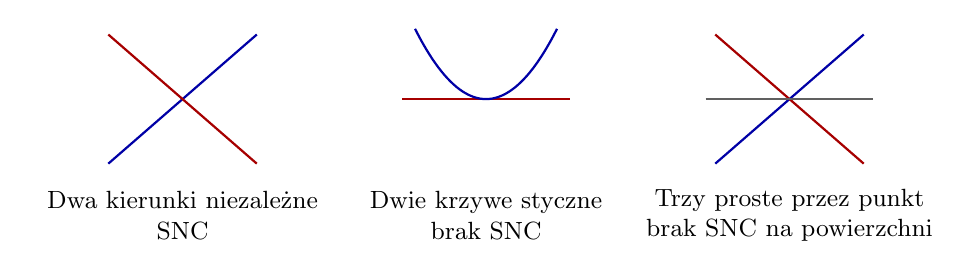
\begin{tikzpicture}[scale=0.82,every node/.style={font=\small}]
 \begin{scope}[shift={(-4.7,0)}]
   \draw[thick,blue!65!black] (-1.15,-1.0)--(1.15,1.0);
  \draw[thick,red!65!black] (-1.15,1.0)--(1.15,-1.0);
  \node[align=center,text width=3.7cm] at (0,-1.8)
  {Dwa kierunki niezależne\\SNC};
 \end{scope}
 \begin{scope}
  \draw[thick,red!65!black] (-1.3,0)--(1.3,0);
  \draw[domain=-1.1:1.1,smooth,variable=\t,thick,blue!65!black]
   plot ({\t},{0.9*\t*\t});
  \node[align=center,text width=3.7cm] at (0,-1.8)
  {Dwie krzywe styczne\\brak SNC};
 \end{scope}
 \begin{scope}[shift={(4.7,0)}]
  \draw[thick,blue!65!black] (-1.15,-1.0)--(1.15,1.0);
  \draw[thick,red!65!black] (-1.15,1.0)--(1.15,-1.0);
  \draw[thick,gray!75!black] (-1.3,0)--(1.3,0);
  \node[align=center,text width=3.7cm] at (0,-1.8)
  {Trzy proste przez punkt\\brak SNC na powierzchni};
 \end{scope}
\end{tikzpicture}

{\small Rysunek 5.3. Trzy lokalne konfiguracje dzielników zredukowanych na gładkiej powierzchni. Dopuszczalne są tylko proste skrzyżowania normalne, jak w lewym panelu.}\par
\end{center}

\begin{twierdzenie}[Trzy rozdmuchania dają rozwiązanie zanurzone ostrza]
\label{tw:ga5-embedded-cusp}
Dla krzywej $C=\V(y^2-x^3)$ w gładkiej powierzchni
$\A^2_k$ istnieje ciąg trzech rozdmuchań w punktach,
po którym transformata ścisła $C^{(3)}$ jest gładka,
a zredukowana suma $C^{(3)}$ i dzielników wyjątkowych
ma proste skrzyżowania normalne. Pierwsze rozdmuchanie
wygładza samą krzywą, ale nie wystarcza do SNC.
\end{twierdzenie}
\begin{proof}
\emph{Krok 1.} Współrzędne pierwszej mapy to
$(x,v)$, $y=xv$. Transformata ścisła ma równanie
$C^{(1)}:\ x=v^2$, a pierwszy dzielnik wyjątkowy
$E_1:\ x=0$. Obie krzywe są gładkie i styczne
w $(0,0)$. Dlatego rozdmuchujemy ten punkt.

\emph{Krok 2.} Na mapie drugiego rozdmuchania,
w którym $x=vw$, mamy
$C^{(1)}:\ vw=v^2$. Po usunięciu czynnika
wyjątkowego $v$ otrzymujemy
$C^{(2)}:\ w=v$. Nowy dzielnik wyjątkowy ma
równanie $E_2:\ v=0$, a transformata ścisła
poprzedniego dzielnika $E_1:\ x=0$ ma równanie
$E_1':\ w=0$. Zatem przez początek mapy
przechodzą \emph{trzy} różne gładkie krzywe
$w=v$, $v=0$ i $w=0$. Każde dwie przecinają się
transwersalnie, ale ich suma nie jest SNC na powierzchni.
Na drugiej mapie tego rozdmuchania, gdzie $v=xu$,
transformata ścisła $C^{(2)}$ spełnia $xu^2=1$,
więc nie ma tam punktu nad rozdmuchiwanym centrum.
Wszystkie pozostałe przecięcia rozważanych krzywych
były już SNC lub nie występowały.

\emph{Krok 3.} Rozdmuchujemy jedyny punkt potrójny
$(v,w)=(0,0)$. Na mapie $v=a$, $w=ab$
transformata $C^{(2)}$ spełnia
$a(b-1)=0$, zatem jej transformata ścisła ma
równanie $b=1$. Nowy dzielnik wyjątkowy ma
równanie $E_3:\ a=0$, natomiast transformata $E_1'$
ma równanie $b=0$. Krzywa $C^{(3)}$ przecina
$E_3$ w $(a,b)=(0,1)$, gdzie $E_1''$ nie przechodzi.
Przecięcie jest transwersalne, ponieważ lokalne
równania $a=0$ oraz $b-1=0$ mają niezależne
różniczki $da$ i $db$.

Na drugiej mapie $v=wc$, $w=d$ transformata
$E_2$ ma równanie $c=0$, a $E_3$ ma równanie
$d=0$; przecinają się transwersalnie. W tej mapie
$C^{(3)}$ spełnia $1=c$, więc przecina $E_3$
w punkcie $(d,c)=(0,1)$, który jest tym samym
punktem co $(a,b)=(0,1)$ w poprzedniej mapie:
na przecięciu $c=1/b$, a $b=1$.
Transformata $E_1''$ nie przechodzi przez ten punkt,
bo w pierwszej mapie ma $b=0$. Spotkania
$E_1''$ z $E_3$ i $E_2''$ z $E_3$ zachodzą
w dwóch innych punktach, odpowiadających różnym
kierunkom $[v:w]$, i każde jest transwersalne.
Nie ma już przecięć potrójnych ani stycznych.
Zatem zredukowany całkowity dzielnik ma SNC.
\end{proof}

\begin{uwaga}[Uwaga o krotnościach dzielnika całkowitego]
Po kolejnych podstawieniach transformata \emph{całkowita}
równania $y^2-x^3$ ma wielokrotne składowe wyjątkowe.
Po drugim rozdmuchaniu jej lokalne równanie to
$v^3w^2(v-w)=0$, a po trzecim (w mapie $v=a$,
$w=ab$) ma postać $a^6b^2(1-b)=0$.
Warunek SNC w poprzednim twierdzeniu dotyczy
\emph{nośnika zredukowanego} dzielnika całkowitego,
nie twierdzi, że jego składowe występują z krotnością jeden.
W teorii rozwiązywania osobliwości ta różnica jest
kluczowa dla obliczeń rozbieżności, całek lokalnych
i niezmienników singularności.
\end{uwaga}

\begin{przyklad}[Taknod: po pierwszym rozdmuchaniu problem nie znika]
Niech $C=\V(y^2-x^4)$. Nad $k$ o charakterystyce
różnej od $2$ ma dwie gałęzie $y=x^2$ i $y=-x^2$,
styczne do siebie w początku. Po podstawieniu
$y=xv$ otrzymujemy transformatę ścisłą
$v^2-x^2=(v-x)(v+x)=0$. Są to dwie gładkie,
przecinające się gałęzie, ale obie przechodzą
przez ten sam punkt pierwszego dzielnika wyjątkowego.
Drugie rozdmuchanie rozdziela ich kierunki
$v=x$ i $v=-x$, dzięki czemu obie transformaty
spotykają nowy dzielnik wyjątkowy w różnych punktach.
Jest to przykład, w którym zmniejszanie krotności
równania nie jest tym samym co zakończenie
rozwiązywania zanurzonego.
\end{przyklad}

\subsection{Normalizacja a rozdmuchanie krzywej}

\begin{stwierdzenie}[Ostrze i węzeł: normalizacje policzone jawnie]
\label{st:ga5-normalization}
Niech $k$ będzie ciałem algebraicznie domkniętym
charakterystyki różnej od $2$. Wówczas:
\begin{enumerate}[label=(\roman*)]
\item normalizacją $k[x,y]/(y^2-x^3)$ jest $k[t]$
przy $x=t^2$, $y=t^3$;
\item normalizacją $k[x,y]/(y^2-x^2-x^3)$ jest
$k[t]$ przy $x=t^2-1$, $y=t(t^2-1)$.
\end{enumerate}
W obu przypadkach transformata ścisła po pierwszym
rozdmuchaniu płaszczyzny jest izomorficzna z $\A^1_t$
i realizuje tę normalizację. Preobrazy punktu osobliwego
mają odpowiednio jeden punkt $t=0$ oraz dwa punkty
$t=1$ i $t=-1$.
\end{stwierdzenie}
\begin{proof}
W (i) z równania $y^2=x^3$ wynika w ciele ułamków
$t=y/x$, $t^2=x$ oraz $t^3=y$. Zatem
$A\subseteq k[t]\subseteq\Frac(A)$ i $t$ jest całkowity
nad $A$, bo spełnia równanie moniczne $T^2-x=0$.
W szczególności $k[t]$ jest skończonym modułem nad
$A$, generowanym przez $1,t$. Jest całkowicie
domknięty, bo $k[t]$ to pierścień euklidesowy.
Jeżeli $s\in\Frac(A)$ jest całkowity nad $A$, to jest
też całkowity nad $k[t]$ (to samo równanie moniczne
ma współczynniki w $k[t]$), więc $s\in k[t]$.
Stąd $k[t]$ jest domknięciem całkowitym $A$.
Porównanie ze wzorami z przykładu~\ref{prz:ga5-cusp}
pokazuje, że jest też pierścieniem transformaty ścisłej.

W (ii) podobnie $t=y/x$ spełnia $t^2=1+x$,
skąd $x=t^2-1$, $y=t(t^2-1)$; zatem
$A\subseteq k[t]\subseteq\Frac(A)$, a $t$ jest
całkowity nad $A$. Ten sam argument daje normalizację.
W pierwszej mapie rozdmuchania relacja
$x=v^2-1$ pokazuje, że transformata ścisła ma
pierścień $k[v]$ i odpowiada $t=v$.
Ostatnie twierdzenie o włóknach to bezpośrednie
rozwiązanie równań $t^2=0$ oraz $t^2-1=0$.
\end{proof}

\begin{przyklad}[Schematowe przecięcie a liczba gałęzi]
Dla węzła $y^2=x^2+x^3$ transformata ścisła po
rozdmuchaniu ma w mapie $y=xv$ równanie
$x=v^2-1$. Jej przecięcie z dzielnikiem wyjątkowym
$x=0$ ma pierścień $k[v]/(v^2-1)\cong k\times k$
(przy $\operatorname{char}k\ne2$): dwa różne punkty
zredukowane. Dla ostrza $y^2=x^3$ analogiczny
pierścień wynosi $k[v]/(v^2)$: jeden punkt
niezredukowany długości dwa. Równość sumy krotności
przecięć nie oznacza więc równości liczby gałęzi.
Ten rachunek pokazuje, dlaczego nie wolno zastępować
przecięcia schematowego samym zbiorem punktów.
\end{przyklad}

\begin{uwaga}[Dlaczego normalizacja nie rozwiązuje wszystkiego?]
Normalizacja jest skończonym morfizmem biwymiernym
z przestrzeni normalnej; dla krzywych skończonego typu
nad ciałem doskonałym normalność oznacza gładkość.
W wyższych wymiarach \emph{normalność nie oznacza
gładkości}. Na przykład stożek kwadratowy
$z^2=x^2+y^2$ w $\A^3_\C$ ma izolowaną osobliwość
w początku, mimo że jego pierścień współrzędnych
jest normalny (można to sprawdzić kryterium Serre'a
$R_1+S_2$, którego tu nie dowodzimy).
Dlatego rozwiązywanie osobliwości powierzchni
wymaga więcej niż samej normalizacji.
\end{uwaga}

\section{Przypadek wyższych wymiarów: gładkie centra i stożek}
\label{sec:ga5-higherdim}

\begin{twierdzenie}[Rozdmuchanie przestrzeni afinicznej wzdłuż podprzestrzeni]
\label{tw:ga5-smooth-center-model}
Niech $1\le c\le n$ i niech
$X=\A^n_k=\Spec k[x_1,\ldots,x_n]$.
Dla centrum $Z=\V(x_1,\ldots,x_c)$ rozdmuchanie
$\widetilde X=\operatorname{Bl}_Z X$ jest gładkie.
Na mapie odpowiadającej $x_i$, $1\le i\le c$,
ma współrzędne
\[
 x_i,\quad u_j=x_j/x_i\ (1\le j\le c,\ j\ne i),
 \quad x_{c+1},\ldots,x_n.
\]
Dzielnik wyjątkowy w tej mapie jest zadany
przez $x_i=0$. Dla każdego punktu $z\in Z$ włókno
$\widetilde X\times_X\Spec\kappa(z)$ jest izomorficzne
z $\PP^{c-1}_{\kappa(z)}$. W szczególności dla punktów
$k$-wymiernych jest to $\PP^{c-1}_k$.
\end{twierdzenie}
\begin{proof}
Z definicji algebry Reesa mapy mają postać
$k[x_1,\ldots,x_n][x_j/x_i:1\le j\le c]$.
Po zastąpieniu $x_j$ przez $x_i u_j$ dla $j\ne i$
otrzymujemy pierścień wielomianów w dokładnie
$n$ algebraicznie niezależnych zmiennych podanych
w tezie. Otrzymujemy otwarty podschemat izomorficzny
z $\A^n_k$, a więc gładki.
Ideał centrum staje się $(x_i)$ i wyznacza dzielnik
$x_i=0$. Po nałożeniu relacji $x_1=\cdots=x_c=0$
na wszystkie mapy pozostaje kolekcja współrzędnych
$u_j$ z przejściami jak dla $\PP^{c-1}$,
niezależna od pozostałych współrzędnych centrum.
Zatem $E\cong Z\times\PP^{c-1}$ w tym liniowym modelu.
\end{proof}

\begin{wniosek}[Gładkie centrum w gładkiej przestrzeni]
\label{wn:ga5-smooth-center}
Niech $X$ i $Z\subseteq X$ będą gładkimi rozmaitościami
algebraicznymi nad ciałem $k$ charakterystyki $0$,
a zanurzenie $Z\hookrightarrow X$ ma stały kowymiar $c$.
Wtedy $\operatorname{Bl}_Z X$ jest gładkie, a jego
dzielnik wyjątkowy jest lokalnie nad $Z$ wiązką
przestrzeni rzutowych, której włókno nad $z\in Z$
jest izomorficzne z $\PP^{c-1}_{\kappa(z)}$.
\end{wniosek}
\begin{proof}
Potrzebny jest standardowy lokalny model zanurzenia
gładkiego: w otoczeniu étale każdego punktu $Z$
para $(X,Z)$ jest równoważna parze
$(\A^n,\A^{n-c})$, z centrum wyznaczonym przez
pierwszych $c$ współrzędnych. Jest to geometryczna
wersja algebraicznego twierdzenia o funkcji uwikłanej.
Rozdmuchanie jest zgodne z płaską zmianą bazy
(twierdzenie~\ref{tw:ga5-flat-basechange} poniżej),
a morfizmy étale są płaskie. Po tej zmianie bazy
mapy mają postać z poprzedniego twierdzenia.
Gładkość jest lokalna w topologii étale, zatem
$\operatorname{Bl}_Z X$ jest gładkie. Mapy współrzędnych dzielnika
wyjątkowego sklejają się do projektywizacji wiązki
normalnej. Przyjęty zewnętrzny składnik dowodu to
wskazane twierdzenie o lokalnym modelu étale;
nie jest ono ukryte w rachunku współrzędnych.
\end{proof}

\begin{przyklad}[Rozdmuchanie prostej w $\A^3$]
Dla $X=\A^3_{x,y,z}$ i $Z=\{x=y=0\}$
mamy $I=(x,y)$. Na mapie $y=xv$ współrzędnymi
są $(x,v,z)$, a dzielnik wyjątkowy ma równanie
$x=0$. Nad każdym punktem $(0,0,z_0)$ w centrum
pojawia się $\PP^1$. Różnica wobec rozdmuchania
punktu jest taka, że dzielnik wyjątkowy jest teraz
powierzchnią, nie krzywą.
\end{przyklad}

\begin{przyklad}[Rozwiązanie izolowanej osobliwości stożka]
\label{prz:ga5-cone}
Niech $X\subseteq\A^3_k$ będzie dane przez
$z^2=x^2+y^2$. W charakterystyce różnej od $2$
pochodne równania to $-2x,-2y,2z$, więc jedynym
punktem osobliwym jest początek. Rozdmuchujemy
\emph{przestrzeń otaczającą} $\A^3$ w początku
i bierzemy transformatę ścisłą $X$.

Na mapie $x\ne0$ kierunku (nie należy mylić tego
z warunkiem $x\ne0$ na samej przestrzeni rozdmuchanej)
piszemy $y=xu$, $z=xv$; transformata ścisła ma
równanie $v^2=1+u^2$. Jej gradient względem
$(u,v)$ to $(-2u,2v)$, który nie może się zerować
na krzywej $v^2-u^2=1$.

Na mapie kierunku $z\ne0$ piszemy
$x=za$, $y=zb$ i otrzymujemy $1=a^2+b^2$,
również gładkie równanie; mapa kierunku $y\ne0$
jest analogiczna do pierwszej mapy. Cała transformata
ścisła jest więc gładką powierzchnią.
Jej przecięcie z wyjątkową $\PP^2$ jest stożkową
$[X:Y:Z]\in\PP^2$ o równaniu $Z^2=X^2+Y^2$,
gładką, a zatem izomorficzną z $\PP^1$.
To pokazuje, jak jeden punkt osobliwy powierzchni
zostaje zastąpiony całą gładką krzywą.
\end{przyklad}

\section{Zmiana bazy, geometria biwymierna i granice metody}
\label{sec:ga5-basechange}

\begin{twierdzenie}[Rozdmuchanie i płaska zmiana bazy]
\label{tw:ga5-flat-basechange}
Niech $A\to B$ będzie homomorfizmem płaskim,
a $I\subseteq A$ ideałem skończenie generowanym.
Wówczas istnieje naturalny izomorfizm schematów nad
$\Spec B$:
\[
 \operatorname{Bl}_{IB}\Spec B\cong
 \operatorname{Bl}_{I}\Spec A\times_{\Spec A}\Spec B.
\]
Analogiczne twierdzenie zachodzi dla płaskiej zmiany
bazy dowolnych schematów i quasi-koherentnych
snopów ideałów skończonego typu.
\end{twierdzenie}
\begin{proof}
Z płaskości wynika, że po zastosowaniu iloczynu tensorowego z $B$
każdy dokładny ciąg
$0\to I^n\to A\to A/I^n\to0$ pozostaje dokładny.
Stąd $I^n\otimes_A B$ identyfikuje się z ideałem
$I^nB=(IB)^n\subseteq B$. Mamy zatem izomorfizm
stopniowanych $B$-algebr
\[
 \mathcal R_A(I)\otimes_A B\cong
 \bigoplus_{n\ge0}(IB)^nT^n=\mathcal R_B(IB).
\]
Po zastosowaniu $\operatorname{Proj}$, który zachowuje
zmianę bazy, otrzymujemy izomorfizm z tezy.
Dla schematów argument stosujemy na afinicznych
otwartych i sklejamy otrzymane izomorfizmy.
\end{proof}

\begin{uwaga}[Dlaczego płaskość jest ważna?]
Bez płaskości odwzorowanie $I^n\otimes_A B\to B$
może mieć niezerowe jądro. Nie ma wówczas podstaw,
by utożsamiać wyrazy algebry Reesa po zmianie bazy
z potęgami ideału $IB$. Dlatego twierdzenie nie mówi,
że rozdmuchanie komutuje z \emph{dowolną} zmianą bazy.
\end{uwaga}

\begin{przyklad}[Konkretny brak zgodności przy zmianie bazy]
Niech $A=k[x,y]$, $I=(x,y)$ oraz
$B=A/(x)\cong k[y]$. Gdyby zmiana bazy była zawsze
zgodna z rozdmuchaniem, dostalibyśmy rozdmuchanie
prostej $\Spec k[y]$ w centrum $(y)$, które jest
izomorfizmem (wniosek~\ref{wn:ga5-cartier-trivial}).
Tymczasem
$\operatorname{Bl}_{(x,y)}\A^2\times_{\A^2}\V(x)$
na pierwszej mapie $y=xv$ spełnia po podstawieniu
$x=0$ także $y=0$, więc pozostaje cały
otwarty podschemat $\Spec k[v]$, odwzorowywany w początek.
Na drugiej mapie $x=uy$ po podstawieniu $x=0$
dostajemy równanie $uy=0$: oprócz transformaty
prostej $u=0$ znajduje się składowa wyjątkowa
$y=0$. Jest to większy schemat niż sama prosta.
\end{przyklad}

\begin{uwaga}[Wyjątkowość, samoprzecięcie i znak minus]
Dla rozdmuchania gładkiej powierzchni w punkcie
$E\cong\PP^1$ oraz
$\mathcal O_{\widetilde X}(E)|_E\cong\mathcal O_{\PP^1}(-1)$.
Gdy powierzchnia jest właściwa i ma zdefiniowane
liczby przecięcia, wynika stąd $E\cdot E=-1$.
Znak minus jest ważny w klasyfikacji powierzchni:
krzywe wyjątkowe pierwszego rodzaju można następnie
\emph{zdmuchiwać} (ang. \emph{blow-down}).
Nie traktujemy tu tego faktu jako udowodnionego:
wymaga teorii wiązek normalnych i liczb przecięcia,
którą rozwiniemy w rozdziałach o powierzchniach
i teorii przecięć.
\end{uwaga}

\subsection{Co mówi twierdzenie Hironaki?}

\begin{twierdzenie}[Hironaka: istnienie rozwiązania osobliwości,
wersja w charakterystyce zero]
\label{tw:ga5-hironaka}
Niech $k$ będzie ciałem charakterystyki $0$, a $X$
zredukowanym, rozdzielonym schematem skończonego typu nad $k$.
Wówczas istnieje właściwy morfizm
$\pi:\widetilde X\to X$ z gładkiego schematu
$\widetilde X$, który jest izomorfizmem nad gładkim
miejscem $X$ i jest biwymierny na każdej składowej
nierozkładalnej. W wersji zanurzonej dla zredukowanej
hiperpowierzchni $D$ w gładkiej rozmaitości $M$
można uzyskać ten efekt poprzez skończony ciąg
rozdmuchań odpowiednio dobranych gładkich centrów,
tak aby transformata ścisła $D$ była gładka, a
zredukowana suma transformaty ścisłej i dzielników
wyjątkowych miała proste skrzyżowania normalne.
\end{twierdzenie}

\begin{uwaga}[Granica samodzielności: status dowodu]
Nie podajemy tu dowodu pełnego twierdzenia Hironaki.
W przeciwieństwie do obliczeń krzywych płaskich nie jest
to konsekwencja kilku podstawień współrzędnych.
Konstrukcja wymaga wyboru centrów na podstawie
zmniejszających się niezmienników osobliwości,
kontroli ich zachowania przy rozdmuchaniach
i indukcji po wymiarze oraz po tych niezmiennikach.
Powyższy wynik cytujemy jawnie jako twierdzenie
zewnętrzne. Udowodniliśmy natomiast bezpośrednio
wszystkie szczególne obliczenia ostrza, węzła
i stożka podane w tym rozdziale.
\end{uwaga}

\begin{uwaga}[Dlaczego charakterystyka zero nie jest ozdobnikiem?]
W dodatniej charakterystyce istnieją rozległe
teorie rozwiązywania osobliwości w niskich wymiarach,
jednak pełna wersja twierdzenia w dowolnym wymiarze
nie jest znana w tej ogólności. W rachunku
współrzędnych dodatnia charakterystyka może powodować
znikanie pochodnych potęg $p$; w metodzie globalnej
trudniejszym problemem jest zachowanie wielkości
mierzących złożoność osobliwości po rozdmuchaniu.
\end{uwaga}

\begin{uwaga}[Rozdmuchania a biracjonalność]
Gdy centrum nie zawiera żadnej składowej $X$, rozdmuchanie
jest izomorfizmem nad gęstym otwartym podzbiorem
$X\setminus Z$, a zatem jest morfizmem biwymiernym,
gdy $X$ jest całkowity. Nie każdy morfizm biwymierny
jest pojedynczym rozdmuchaniem, a nie każda
biracjonalna modyfikacja ma postać rozdmuchania
gładkiego centrum. Rozkładanie ich na elementarne
operacje to osobny problem geometrii biwymiernej.
\end{uwaga}

\section{Mapa pojęć i perspektywa następnego rozdziału}
\label{sec:ga5-outlook}

W rozdziale przeprowadziliśmy następujący łańcuch idei:
\emph{ideał centrum $I$ $\longrightarrow$ potęgi $I^n$
$\longrightarrow$ algebra Reesa $\longrightarrow$
$\operatorname{Proj}$ $\longrightarrow$ rozdmuchanie
$\longrightarrow$ transformaty i dzielniki wyjątkowe}.
Właściwość uniwersalna mówi, że rozdmuchanie jest
kanoniczną operacją czyniącą ideał centrum odwracalnym.
W praktyce na gładkich powierzchniach rachunek ten
sprowadza się do dwóch prostych podstawień
$y=xv$ i $x=yu$. Dopiero śledzenie przecięć
z dzielnikami wyjątkowymi wyjaśnia, ile takich operacji
trzeba wykonać, aby uzyskać konfigurację SNC.

\begin{center}
\begin{minipage}{\linewidth}
\centering
\begin{tikzpicture}[>=Stealth,node distance=9mm,
 every node/.style={font=\small},
 b/.style={draw,rounded corners,align=center,text width=7.8cm,inner sep=5pt}]
 \node[b] (a) {Centrum $Z=\V(\mathcal I)$ i filtracja $\mathcal I^0,\mathcal I^1,\ldots$};
 \node[b,below=of a] (b1) {Algebra Reesa $\mathcal R(\mathcal I)=\bigoplus_{n\ge0}\mathcal I^nT^n$};
 \node[b,below=of b1] (c) {$\widetilde X=\operatorname{Proj}_X\mathcal R(\mathcal I)$,\quad $E=\operatorname{Proj}_Z\operatorname{gr}_{\mathcal I}(\mathcal O_X)$};
 \node[b,below=of c] (d) {Mapy współrzędnych $y=xv$, $x=yu$: transformata całkowita i ścisła};
 \node[b,below=of d] (e) {Rozwiązanie osobliwości\\oraz proste skrzyżowania normalne (SNC)};
 \draw[->,thick] (a)--(b1);
 \draw[->,thick] (b1)--(c);
 \draw[->,thick] (c)--(d);
 \draw[->,thick] (d)--(e);
\end{tikzpicture}

{\small Rysunek 5.4. Logiczna zależność pojęć, a nie algorytm automatycznego rozwiązywania wszystkich osobliwości.}\par
\end{minipage}
\end{center}

\begin{przyklad}[Dwa kolejne rozdmuchania ostrza $y^2=x^5$]
Rozważmy krzywą $C=\V(y^2-x^5)\subset\A^2_{\C}$.
W mapie $y=xv$ pierwszego rozdmuchania mamy
$y^2-x^5=x^2(v^2-x^3)$. Dzielnik wyjątkowy jest
określony równaniem $x=0$, a transformata ścisła
$C_1$ ma równanie $v^2=x^3$. W szczególności
$C_1$ nadal ma ostrze w $(0,0)$: obie pochodne
cząstkowe równania $v^2-x^3$ tam znikają.

Rozdmuchajmy teraz ten punkt. W mapie $v=xw$
otrzymujemy $v^2-x^3=x^2(w^2-x)$, a zatem
transformata ścisła $C_2$ jest dana równaniem
$x=w^2$. Jest ona gładka, ponieważ pochodna
$x-w^2$ względem $x$ jest równa $1$.
Nie wynika stąd jednak, że konfiguracja całkowitego
przeciwobrazu $C$ ma proste skrzyżowania normalne.
Rzeczywiście $C_2$ styka się z nowym dzielnikiem
wyjątkowym $x=0$ w punkcie $(0,0)$, gdyż ograniczenie
$x=w^2$ daje tam przecięcie o krotności $2$.
Jeśli celem jest rozwiązanie zanurzone, należy więc
kontynuować rozdmuchania i kontrolować wszystkie
składowe dzielnika wyjątkowego, nie tylko gładkość $C_2$.
\end{przyklad}

\begin{uwaga}[Przygotowanie do geometrii powierzchni]
W następnym rozdziale rozdmuchania staną się
narzędziem, a nie głównym obiektem. Zajmiemy się
powierzchniami algebraicznymi, przekształceniami
biwymiernymi, ich dzielnikami i krzywymi wyjątkowymi.
W rozdziale o teorii przecięć wyprowadzimy
liczbowy sens $E^2=-1$ i podstawowe formuły
dla przecięć po rozdmuchaniu. Tam również rozróżnimy
równość cykli od równości samych nośników.
\end{uwaga}

% Literatura kontrolna (niewymagana do zrozumienia rachunków):
% The Stacks Project: 01OF (Blowing up), 01V4 (Smooth morphisms),
% 01W7 (Projective morphisms), 0FUT (Blow-up of smooth center).
% Wykorzystane jako odniesienia do twierdzen zewnetrznych:
% Hironaka (resolution in characteristic zero), etale-local smooth centers.


% =========================================================
% ROZDZIAL 6. POWIERZCHNIE ALGEBRAICZNE
% =========================================================
